% MAAI 902 Natural Language Processing & LLMs: Assessment Task 3, Applied NLP Project report (group).
% Upload this folder (with figures/) to Overleaf and compile with pdfLaTeX.
\documentclass[11pt,a4paper]{article}
\usepackage[margin=2.2cm]{geometry}
\usepackage[T1]{fontenc}
\usepackage{mathptmx}
\usepackage{graphicx}
\usepackage{booktabs}
\usepackage{amsmath}
\usepackage[hidelinks]{hyperref}
\setlength{\parskip}{4pt}

\title{What SEC Filings Tell Us About the Next Market Move:\\ Fine-Tuned Transformers, a 7B Financial LLM and an Event Study on 50 US Companies}
\author{Krishna Harsha Tangirala (lead author) \and Mohammed Shahrukh \and Valavala Divya Anu Sri \and Sreeya Tirumalasetti \and Venkata Saisravan Pasam\\[2pt]
\small Master of Applied Artificial Intelligence, University of Wollongong in Dubai\\
\small MAAI 902 Natural Language Processing \& LLMs, Applied NLP Project (group)}
\date{}

\begin{document}
\maketitle

\begin{center}
\small
GitHub repository: \url{https://github.com/harshatangirala/nexus-alpha-v3-university-of-wollongong-in-dubai}\\
NLP dataset (EDGAR filing text and metadata): \url{https://drive.google.com/drive/folders/1nczPvpd_wkMgF5N7uFBfAQMp-Ja96TRI}\\
Lite dashboard (public, always on): \url{https://nexus-alpha-v3-lite.streamlit.app}\\
Full dashboard (heavy, runs on the author's machine): \url{https://anime-sedan-harddisk.ngrok-free.dev}
\end{center}

\section{Problem statement and objectives}

Every listed US company files reports with the Securities and Exchange Commission: an annual 10-K, three quarterly 10-Qs and an 8-K whenever something material happens, such as quarterly results, a merger or a change of chief executive. These documents are public within minutes, they are long, and they are written in a careful legal register that hides news inside boilerplate. Investors read them, and a growing number of products now claim that language models can read them faster and turn the words into trading signals.

That claim is hard to check. Most studies of text and returns either use news headlines, test on a period the language model may have seen during pre-training, or skip the controls that would separate what a filing says from who filed it and when. A filing always reveals the company, and a company's typical behaviour is itself predictive, so a model can look clever while learning nothing from the words.

Our project asks two questions with a design that tries to close those gaps. First, which filings actually move prices, and by how much? Second, can modern language models, from a TF-IDF baseline through fine-tuned BERT-family encoders to a 7-billion-parameter financial LLM, forecast what happens next from the text alone? The objectives were:

\begin{itemize}
\item O1. Build a point-in-time corpus of 10-K, 10-Q and 8-K filings for 50 large US companies, 2016 to 2026, with acceptance timestamps.
\item O2. Measure the price reaction to each filing type against matched days without a filing (an event study).
\item O3. Fine-tune and compare six language models plus a TF-IDF baseline on identical filings for direction, volatility and the risk of a fall greater than 10\%, at 5, 10, 20 and 40 trading sessions.
\item O4. Test whether any text signal survives once company identity, the filing calendar and simple price features are controlled for.
\item O5. Deploy the result in a web application with a grounded LLM assistant that explains each forecast in plain language.
\end{itemize}

The study is one half of a multimodal project. The other half reads candlestick charts with vision networks, and the dashboard combines both. This report covers the language side.

\section{Dataset description and pre-processing}

\textbf{Sources and collection.} Filings were downloaded from SEC EDGAR under the SEC fair-access policy, with a declared user agent and at most eight requests per second. The universe is the same 50 companies used on the vision side, ten in each of five sectors. Prices come from verified intraday bars, which let us place each filing at the first tradeable moment after it became public.

\textbf{Size.} The corpus holds 10,269 filings: 554 10-Ks, 1,700 10-Qs and 8,015 8-Ks. Counts are steady at about 50 annual and 150 quarterly reports a year, while 8-Ks fall from roughly 800 a year before 2021 to about 600 in 2024 and 2025. Financials file almost twice as many 8-Ks as any other sector (2,518), which matters later because it gives that sector more training examples. Table~\ref{tab:corpus} summarises the text.

\begin{table}[h]
\centering
\caption{The corpus by form: number of filings, median length in characters and how often the MD\&A section was found.}
\label{tab:corpus}
\begin{tabular}{lrrrr}
\toprule
Form & Filings & Median document & Median section used & MD\&A found \\
\midrule
10-K (annual) & 554 & 381,688 & 83,366 & 85.0\% \\
10-Q (quarterly) & 1,700 & 153,539 & 53,069 & 89.3\% \\
8-K (current events) & 8,015 & 8,233 & 8,233 & not applicable \\
\bottomrule
\end{tabular}
\end{table}

\textbf{Timestamps.} Look-ahead bias is the main way a filing study goes wrong, so time handling got more care than anything else. The acceptance time comes from the filing's SGML header, or from the later of two JSON readings when the header is missing. A filing counts as available 35 minutes after acceptance, and the trade enters at the first hourly bar after that. Labels are measured from that entry price, never from the day's open.

\textbf{Text extraction.} For 10-K and 10-Q reports we extracted Management's Discussion and Analysis (MD\&A), the section where managers explain results in their own words. Banks often place it in Exhibit 13, which the extractor checks. When no MD\&A heading was found, the full document was used and the fallback was logged. For 8-Ks we used the body plus the EX-99 press release, which usually carries the actual news. HTML was stripped, whitespace collapsed, and every input was written as ``[form] [section] text'', so a model always knows what kind of document it is reading.

\textbf{Tokenisation and length.} Each encoder uses its own sub-word tokenizer. The 512-token models read the first 512 tokens in the fine-tuned setting and four chunks of 512 tokens in the frozen setting, Longformer reads up to 4,096 tokens, and TF-IDF works on word n-grams of the whole section. Length is a real constraint: a median 10-K section of 83,366 characters is roughly 20,000 tokens, far beyond any of these windows.

\textbf{Labels and splits.} Each filing event gets the same twelve targets as the vision models: direction (DOWN, SIDEWAYS or UP, with a sideways band scaled by the stock's own volatility), log realised volatility and a fall of more than 10\%, each at four horizons. Events were split by time into training (2016 to 2020), an early-stopping block (2021), validation (2022--2023) and a locked test (January 2024 to August 2026), with a 40-session gap between blocks. The test holds 2,165 events, opened once after every choice had been frozen and hashed.

\section{Solution architecture}

Fig.~\ref{fig:arch} shows the full system. The language branch has five stages: collection, extraction and event building, seven text models, calibration and combination, and the user-facing application.

\begin{figure}[h]
\centering
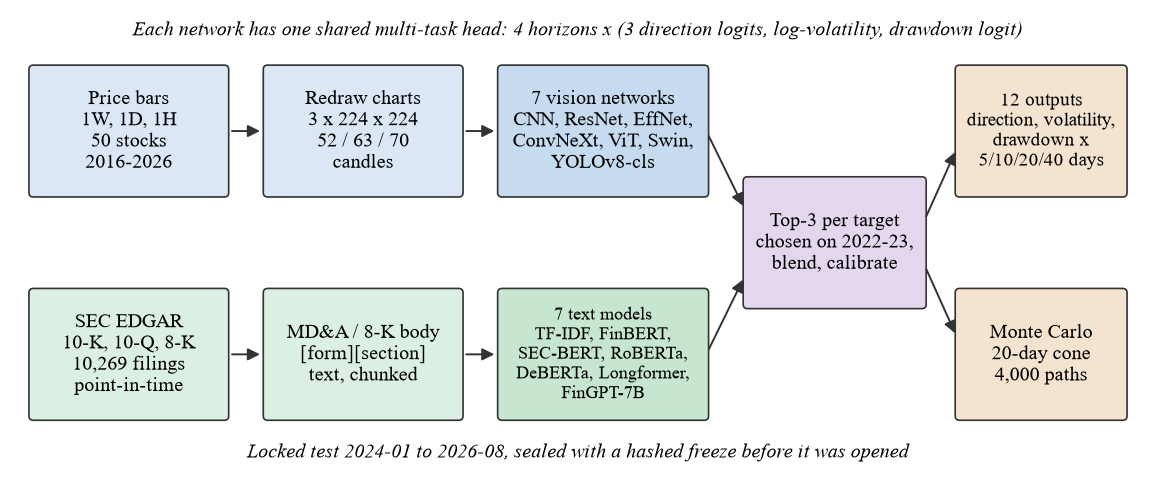
\includegraphics[width=\textwidth]{figures/fig_architecture.png}
\caption{System architecture. The lower branch is the language pipeline described in this report; the upper branch is the vision pipeline; both feed one calibrated combination and the dashboard.}
\label{fig:arch}
\end{figure}

\textbf{Text models.} We chose models that differ along one axis at a time, so that ablations can say something about why one works better:

\begin{itemize}
\item TF-IDF with logistic or ridge regression, the classical baseline with few effective parameters.
\item FinBERT \cite{araci2019}, a BERT-base model \cite{devlin2019} adapted to financial text, and SEC-BERT \cite{loukas2022}, pre-trained on SEC filings, which together test domain pre-training.
\item RoBERTa-large \cite{liu2019roberta} and DeBERTa-v3-large \cite{he2023deberta}, general models with about three times the parameters, which test size.
\item Longformer-4096 \cite{beltagy2020}, which uses sparse attention to read eight times more text, which tests length.
\item FinGPT \cite{yang2023fingpt}, a LoRA adapter \cite{hu2022lora} on Llama-2-7B \cite{touvron2023}, loaded in 4-bit and kept frozen, which tests whether a generative financial LLM adds anything.
\end{itemize}

All encoders end in the same multi-task head as the vision models: a shared hidden layer followed by direction logits, a volatility value and a drawdown logit for each of the four horizons. The fine-tuned route trains the encoder and head together. The frozen route mean-pools the hidden states of four 512-token chunks, reduces them to 32 principal components and fits regularised linear heads, which is cheap and hard to overfit.

\textbf{Combination.} We tested two ways of joining text and charts after calibration. The research combination averages up to three text models per target, chosen on validation, and blends that average with the chart average using a weight also chosen on validation. Validation gave text no weight for any of the four direction horizons, between a quarter and three quarters of the weight for volatility at 10 to 40 sessions, and all of it for drawdown at 10, 20 and 40 sessions. The dashboard runs a simpler recipe that can be served on a laptop: the three best chart networks per target, blended with the three best deployable text models (fine-tuned encoders up to 600 million parameters, or TF-IDF) whenever the stock filed in the last five sessions.

\textbf{Application and LLM assistant.} The Streamlit dashboard lets a user type a ticker or paste chart screenshots, paste a filing summary, and read the forecasts. Its Ask AI tab uses Google Gemini, a hosted LLM, to explain a result in plain language. We ground the model instead of letting it answer freely: every request carries a system prompt with answering rules, a fact sheet of the study's verified results, the exact model routing per target and the numbers of the user's current analysis. This is retrieval-augmented generation in its simplest form \cite{lewis2020rag}. The knowledge base is a few pages of text, small enough to send whole with every question, so the ``retrieval'' step selects all of it. A vector index would only become worthwhile if the assistant also had to search the filings themselves, which is planned future work. The prompt forbids investment advice and invented numbers, and when a model is retired or busy the app falls back to another Gemini model before the first word is shown.

\textbf{Tool stack.} Hugging Face Transformers and PyTorch for the encoders, scikit-learn for TF-IDF and the linear heads, LightGBM for the numerical baselines, Google Colab GPUs for training, Streamlit and Plotly for the interface, and the Gemini REST API for the assistant. Code, notebook and results are on GitHub.

\section{Model training and fine-tuning details}

The five encoders were fine-tuned on the 4,149 training-block filings with AdamW, for at most three epochs with early stopping on the 2021 filings. A short probe on a training subsample chose between two learning rates per model, and the rate with the lower early-stopping loss was kept (Table~\ref{tab:lr}).

\begin{table}[h]
\centering
\caption{Fine-tuning settings kept by the learning-rate probe, with the best early-stopping loss and probe time.}
\label{tab:lr}
\begin{tabular}{lrrr}
\toprule
Model & Learning rate & Early-stopping loss & Probe (min) \\
\midrule
FinBERT & $2\times10^{-5}$ & 1.453 & 0.11 \\
SEC-BERT & $2\times10^{-5}$ & 1.523 & 0.11 \\
RoBERTa-large & $1\times10^{-5}$ & 1.468 & 0.38 \\
Longformer-4096 & $3\times10^{-5}$ & 1.441 & 4.90 \\
DeBERTa-v3-large & $1.5\times10^{-5}$ & 1.907 & 2.05 \\
\bottomrule
\end{tabular}
\end{table}

All five encoders reached their lowest early-stopping loss after the first epoch, and later epochs only fitted the training block better. DeBERTa-v3-large was unstable: its best loss stayed well above the others and rose again in the second epoch. This is a known problem when large encoders are fine-tuned on a few thousand noisy labels \cite{dodge2020,mosbach2021}, usually tackled with several seeds, longer warm-up and layer-wise learning rates. With one seed per model and short training, we report the frozen features next to the fine-tuned ones as the fairer reading for that model.

FinGPT was used frozen. We loaded the Llama-2-7B base with the FinGPT LoRA adapter in 4-bit precision and took both its embeddings and its own sentiment read-out as features. QLoRA fine-tuning \cite{dettmers2023} was planned but switched off for this run to stay within the GPU budget, and it is the first item in the follow-up protocol.

Raw outputs were calibrated on the 2021 block with temperature scaling for direction, Platt scaling for drawdown and a linear map for volatility. The models trained on filing events were also carried to the daily panel, where each trading day sees the most recent filing, so the text branch can be combined with the charts.

\section{Evaluation and results}

\textbf{Metrics and tests.} Direction is scored by macro-F1, and its skill is measured against a null model that shuffles labels within each month. Volatility uses R-squared, where 0 means no better than predicting the average, and drawdown uses ROC-AUC, where 0.5 is chance. Confidence intervals come from a paired month-block bootstrap \cite{kunsch1989} and every family of twelve tests is Holm-corrected \cite{holm1979}. Results below are on the locked 2024--2026 test unless stated otherwise.

\textbf{Which filings move prices.} The event study is the clearest result (Fig.~\ref{fig:event}). On filing days the mean absolute abnormal move was 1.43 normal-day units, against 0.70 on matched days without a filing, so filings roughly double the reaction (one-sided Mann-Whitney $p < 0.001$). The forms also differ (Kruskal-Wallis $p = 0.006$). Quarterly reports move prices most (1.64), then annual reports (1.52) and 8-Ks (1.37). In the development blocks, 8-K item 2.02 (results of operations) produced a mean move of 2.39 over 1,446 filings; item 2.05 (exit or restructuring costs) came next at 2.22, but on only 15 filings. Communication Services reacted most to quarterly reports and Financials least to 10-Qs and 8-Ks, in development and on the test alike.

\begin{figure}[h]
\centering
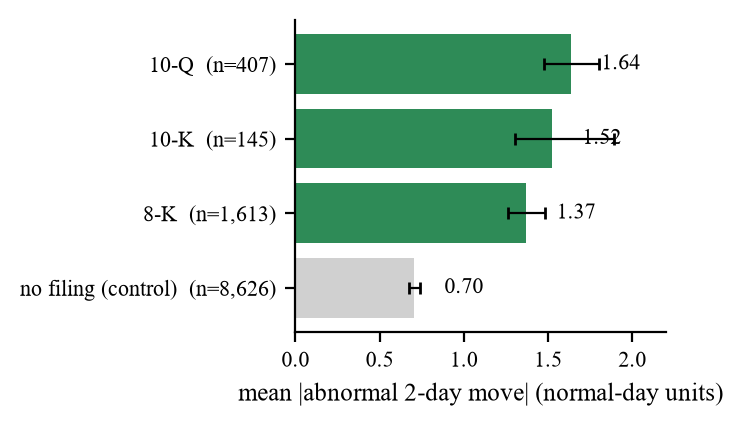
\includegraphics[width=0.62\textwidth]{figures/fig_event_study_test.png}
\caption{Event study on the locked test: mean absolute abnormal two-day move by filing type, with 95\% intervals.}
\label{fig:event}
\end{figure}

\textbf{Can the models forecast from the text?} Against uninformed benchmarks the validation-chosen text models showed skill in none of the four direction tasks, none of the four volatility tasks and all four drawdown tasks, where Longformer reached AUCs between 0.61 and 0.65. Volatility R-squared was negative at every horizon: text alone does not track how volatile a stock is.

The harder test asks whether that drawdown signal survives a no-text baseline on the same filings. Three baselines see the same events without reading them: per-company base rates, a model on momentum and trailing volatility plus the form, and a LightGBM model on 20 technical indicators plus the form. Against the strongest of these, the best text model was better in only 1 of 12 tasks, level in 7 and worse in 4 (all volatility). The single win was SEC-BERT on 20-session direction, about 0.09 macro-F1 above the company base rates. Fig.~\ref{fig:nlp} lays out every model against the baselines.

\begin{figure}[h]
\centering
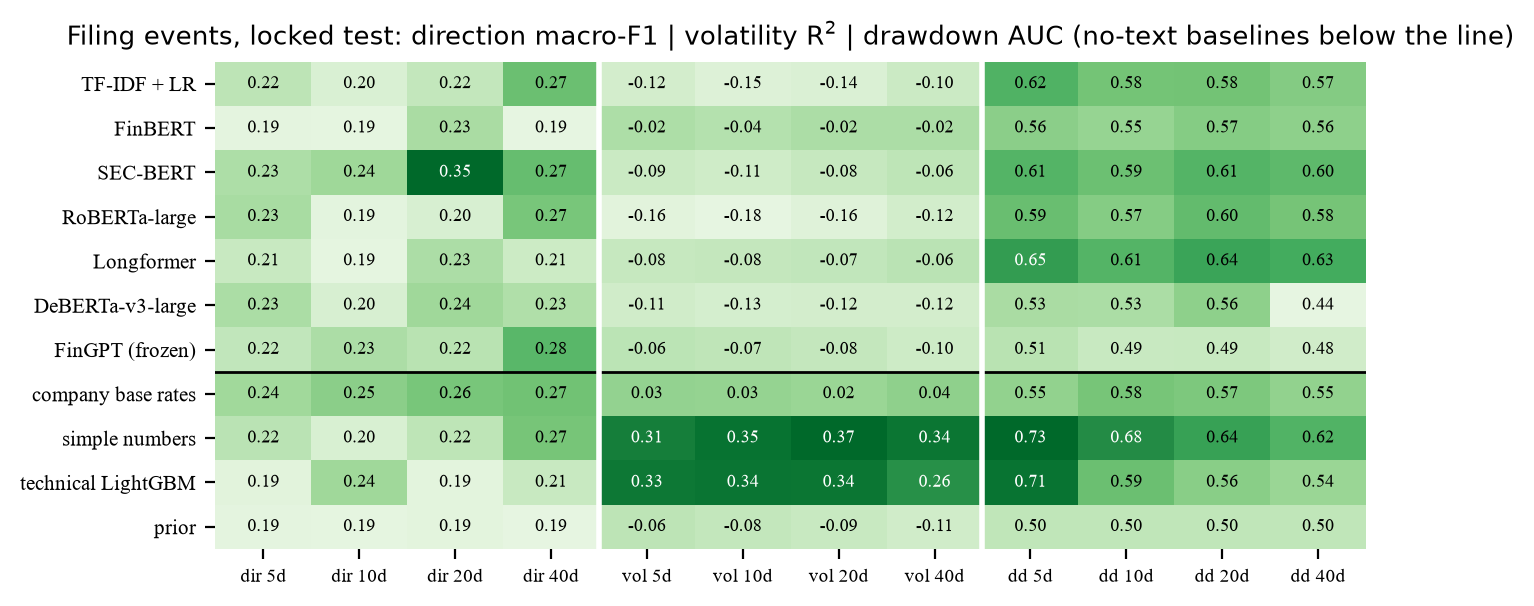
\includegraphics[width=\textwidth]{figures/fig_nlp_events_test.png}
\caption{Locked-test primary metric for every text model (above the line) and the no-text baselines (below) on the same 2,165 filing events.}
\label{fig:nlp}
\end{figure}

\textbf{Shortcut learning.} Several pieces of evidence point the same way. When text features were added to a technical-indicator model on the daily panel, volatility R-squared rose by 0.075 on average. Most of that gain, 0.063, came from the filing-calendar columns alone (how close a day is to an earnings filing). The words added 0.013 beyond the calendar, and 0.007 beyond the calendar and the company. Integrated-gradients attributions \cite{sundararajan2017} for the largest reactions were dominated by dates, company names and formatting tokens. The models mostly learned who filed and when, a textbook case of shortcut learning \cite{geirhos2020}.

\textbf{What the words do explain.} In a regression of the size of the reaction on the filing's form, 8-K items, sector and timing, adding TF-IDF features raised R-squared from 0.181 to 0.235, and the gain stayed at +0.043 (interval 0.029 to 0.058) after the company was controlled for as well. Filing text helps explain how big the market's reaction is, even though it does not predict the direction. Phrases tied to large reactions included ``non-GAAP'' and ``conference call'', the vocabulary of earnings releases. Interpretable measures did less well: Loughran-McDonald tone \cite{loughran2011} and the year-on-year change in a filing's wording \cite{cohen2020} added nothing when put into the no-text model, and FinBERT sentence tone was almost unrelated to the sign of the reaction (Spearman 0.025).

\textbf{Ablations.} With 5,000 bootstrap draws on validation, reading four chunks instead of the first 512 tokens helped frozen encoders on risk targets, for example +0.140 drawdown AUC for RoBERTa-large and +0.101 for SEC-BERT. Length helped Longformer against FinBERT on drawdown (+0.115 AUC). Domain pre-training helped SEC-BERT against FinBERT on direction (+0.067 macro-F1) but cost it 0.148 of volatility R-squared. Fine-tuning against frozen features was mixed: it helped Longformer on drawdown (+0.084) and hurt FinBERT on direction ($-0.034$). Averaging two or three language models never beat the best single one (0 of 12 tasks), which suggests their errors overlap.

\textbf{Text inside the deployed system.} Text matters more as a partner than on its own. Blending the text average into the chart average improved on the charts alone for drawdown at 20 and 40 sessions (+0.090 and +0.061 AUC on the test). The recipe the dashboard actually runs beat its uninformed benchmark in 9 of the 12 test tasks: all four direction horizons, 5-session volatility (R-squared 0.140) and all four drawdown horizons (AUC 0.54 to 0.63).

\textbf{Model ranking.} TF-IDF had the best mean rank on validation (2.92 over 12 tasks), ahead of every transformer. On the test, SEC-BERT ranked first (2.58) and Longformer second (3.08). With about four thousand training filings, a regularised linear model on n-grams is a hard baseline, and differences between close models are better read from intervals than from ranks.

\section{Discussion of ethical issues}

\textbf{Look-ahead bias as an integrity issue.} A language model that memorised news from its pre-training period can appear to forecast it \cite{glasserman2023,sarkar2024}. Our test period starts after the pre-training cut-off of every model we used, every timestamp is point-in-time, and the test labels sat in a hashed vault that logged each opening. Analyses added after the test was opened are labelled post-hoc, so a reader can tell confirmatory from exploratory claims.

\textbf{Bias and shortcut learning.} The models learned company identity and the filing calendar, which is a form of bias: forecasts for a company are partly a replay of its past. Financials, with twice as many 8-Ks, also had more influence on training. We addressed this by testing against per-company and calendar baselines, by reporting results by sector, and by telling the user in the dashboard when a stock is outside the 50 training companies.

\textbf{Privacy and data rights.} Filings are public records and the corpus contains no personal data beyond the names of executives that companies themselves publish, for instance in 8-K item 5.02 on officer changes. We respected EDGAR's fair-access rules. The filing corpus is shared publicly on Google Drive for reproducibility. The intraday price data come from a public dataset without a declared licence, which we state openly; it is used here for non-commercial academic work only. Pre-trained models are used under their own licences, including the Llama 2 Community License for the FinGPT base, and no weights are redistributed.

\textbf{Responsible use of forecasts and of the LLM.} Retail users may treat a confident-looking number as advice. The dashboard shows a direction call only where the locked test supported it, labels drawdown figures as relative risk, and states on every page that this is educational research. The Gemini assistant is the part most likely to mislead, because a fluent answer can sound authoritative. Its prompt restricts it to the study's verified facts, forbids buy or sell advice and invented statistics, and asks it to state its caveat in one plain sentence. Users are told that their questions are sent to Google and may be used on the free tier, so nothing private should be pasted. Testing found a real failure in an earlier version, which answered several questions with ``this was not tested'' when the study had a measured result. Adding the verified results and the per-target model routing to the prompt fixed it.

\textbf{Environmental cost.} The confirmatory run used about 4.2 GPU-hours on one data-centre GPU. Later analyses reused cached predictions and added only CPU time.

\section{Conclusion and lessons learned}

The clearest finding concerns the market's reaction to filings. On the locked test, filing days move prices about twice as much as ordinary days, quarterly reports move them most, and the words of a filing help explain how large the reaction will be beyond the company and the calendar. Forecasting the next move from the text is a different matter. The language models showed skill only on drawdown risk, and that skill did not survive a baseline that knows the company and simple price features. Most of what they learned was who filed and when.

We learned four things we would carry into the next project. Controls matter more than model size: without per-company and calendar baselines, our drawdown result would have looked like a genuine text signal. A TF-IDF model is a serious competitor when labelled data are scarce, and it deserves a place in every comparison. Large encoders need several seeds and careful schedules to fine-tune well on small data. Lastly, a grounded LLM assistant is only as good as the facts it is given, and testing it with awkward questions found errors that a quick demonstration would have missed.

The pre-registered follow-up adds QLoRA fine-tuning of FinGPT, five seeds per model, layer-wise learning-rate decay for the large encoders, minute-stamped news next to filings, and a forward test period starting in December 2026.

\section{Links to GitHub repo and demo}

\begin{itemize}
\item GitHub repository (code, notebook, result tables, dashboard): \url{https://github.com/harshatangirala/nexus-alpha-v3-university-of-wollongong-in-dubai}
\item NLP dataset, EDGAR submissions and extracted filing text with metadata (public Google Drive): \url{https://drive.google.com/drive/folders/1nczPvpd_wkMgF5N7uFBfAQMp-Ja96TRI}
\item All project data, including the price bars used for labels: \url{https://drive.google.com/drive/folders/13rokT8OX1MgZQpzTRLeyvDq-FVdgraSh}
\item Lite dashboard on Streamlit Community Cloud (public): \url{https://nexus-alpha-v3-lite.streamlit.app}. The full dashboard loads 13 networks (2.9 GB of weights, about 5 GB of memory), which is too heavy for free hosting, so the lite version shows the architecture, the evidence, precomputed full-model results for four stocks and the Gemini assistant.
\item Full dashboard (runs on the author's machine through a tunnel, available during demonstrations): \url{https://anime-sedan-harddisk.ngrok-free.dev}
\end{itemize}

\textbf{Team contributions.} Krishna Harsha Tangirala defined the research questions, chose the six language models, the filing types and the targets, ran every Colab execution of the notebook, reviewed each result and audit, decided which post-hoc controls to add and directed the dashboard and its assistant. [Mohammed Shahrukh: role and contribution.] [Valavala Divya Anu Sri: role and contribution.] [Sreeya Tirumalasetti: role and contribution.] [Venkata Saisravan Pasam: role and contribution.]

\textbf{Use of generative AI.} In line with the UOW guidance on acknowledging GenAI, we record that Anthropic's Claude Code wrote most of the code and the Colab notebook and drafted parts of this report under the first author's direction, and that Google Gemini powers the dashboard assistant. Every number reported here comes from the executed notebook's own output files and was checked against them; no data were generated by an AI tool.

\begin{thebibliography}{99}

\bibitem{araci2019} D. Araci, ``FinBERT: Financial sentiment analysis with pre-trained language models,'' arXiv:1908.10063, 2019.

\bibitem{devlin2019} J. Devlin, M.-W. Chang, K. Lee, and K. Toutanova, ``BERT: Pre-training of deep bidirectional transformers for language understanding,'' in \emph{Proc. NAACL-HLT}, 2019, pp. 4171--4186.

\bibitem{loukas2022} L. Loukas \emph{et al.}, ``FiNER: Financial numeric entity recognition for XBRL tagging,'' in \emph{Proc. ACL}, 2022, pp. 4419--4431.

\bibitem{liu2019roberta} Y. Liu \emph{et al.}, ``RoBERTa: A robustly optimized BERT pretraining approach,'' arXiv:1907.11692, 2019.

\bibitem{he2023deberta} P. He, J. Gao, and W. Chen, ``DeBERTaV3: Improving DeBERTa using ELECTRA-style pre-training with gradient-disentangled embedding sharing,'' in \emph{Proc. ICLR}, 2023.

\bibitem{beltagy2020} I. Beltagy, M. E. Peters, and A. Cohan, ``Longformer: The long-document transformer,'' arXiv:2004.05150, 2020.

\bibitem{yang2023fingpt} H. Yang, X.-Y. Liu, and C. D. Wang, ``FinGPT: Open-source financial large language models,'' arXiv:2306.06031, 2023.

\bibitem{hu2022lora} E. J. Hu \emph{et al.}, ``LoRA: Low-rank adaptation of large language models,'' in \emph{Proc. ICLR}, 2022.

\bibitem{touvron2023} H. Touvron \emph{et al.}, ``Llama 2: Open foundation and fine-tuned chat models,'' arXiv:2307.09288, 2023.

\bibitem{lewis2020rag} P. Lewis \emph{et al.}, ``Retrieval-augmented generation for knowledge-intensive NLP tasks,'' in \emph{Advances in Neural Information Processing Systems}, vol. 33, 2020, pp. 9459--9474.

\bibitem{dodge2020} J. Dodge, G. Ilharco, R. Schwartz, A. Farhadi, H. Hajishirzi, and N. Smith, ``Fine-tuning pretrained language models: Weight initializations, data orders, and early stopping,'' arXiv:2002.06305, 2020.

\bibitem{mosbach2021} M. Mosbach, M. Andriushchenko, and D. Klakow, ``On the stability of fine-tuning BERT: Misconceptions, explanations, and strong baselines,'' in \emph{Proc. ICLR}, 2021.

\bibitem{dettmers2023} T. Dettmers, A. Pagnoni, A. Holtzman, and L. Zettlemoyer, ``QLoRA: Efficient finetuning of quantized LLMs,'' in \emph{Advances in Neural Information Processing Systems}, vol. 36, 2023.

\bibitem{kunsch1989} H. R. Künsch, ``The jackknife and the bootstrap for general stationary observations,'' \emph{The Annals of Statistics}, vol. 17, no. 3, pp. 1217--1241, 1989.

\bibitem{holm1979} S. Holm, ``A simple sequentially rejective multiple test procedure,'' \emph{Scandinavian Journal of Statistics}, vol. 6, no. 2, pp. 65--70, 1979.

\bibitem{sundararajan2017} M. Sundararajan, A. Taly, and Q. Yan, ``Axiomatic attribution for deep networks,'' in \emph{Proc. ICML}, PMLR 70, 2017, pp. 3319--3328.

\bibitem{geirhos2020} R. Geirhos \emph{et al.}, ``Shortcut learning in deep neural networks,'' \emph{Nature Machine Intelligence}, vol. 2, no. 11, pp. 665--673, 2020.

\bibitem{loughran2011} T. Loughran and B. McDonald, ``When is a liability not a liability? Textual analysis, dictionaries, and 10-Ks,'' \emph{The Journal of Finance}, vol. 66, no. 1, pp. 35--65, 2011.

\bibitem{cohen2020} L. Cohen, C. Malloy, and Q. Nguyen, ``Lazy prices,'' \emph{The Journal of Finance}, vol. 75, no. 3, pp. 1371--1415, 2020.

\bibitem{glasserman2023} P. Glasserman and C. Lin, ``Assessing look-ahead bias in stock return predictions generated by GPT sentiment analysis,'' arXiv:2309.17322, 2023.

\bibitem{sarkar2024} S. K. Sarkar and K. Vafa, ``Lookahead bias in pretrained language models,'' SSRN Working Paper 4754678, 2024.

\end{thebibliography}

\end{document}
